\subsection{Aplicação Painel: Listagem}
\subsubsection*{Descrição do caso de uso}
Para fazer uma listagem, utilizador apenas necessita de entrar na página. A aparência da \textit{view} deste caso de utilização será semelhante ao demonstrado na figura \ref{fig:di_lista}. 

\begin{figure}[H] 
	\begin{center}
		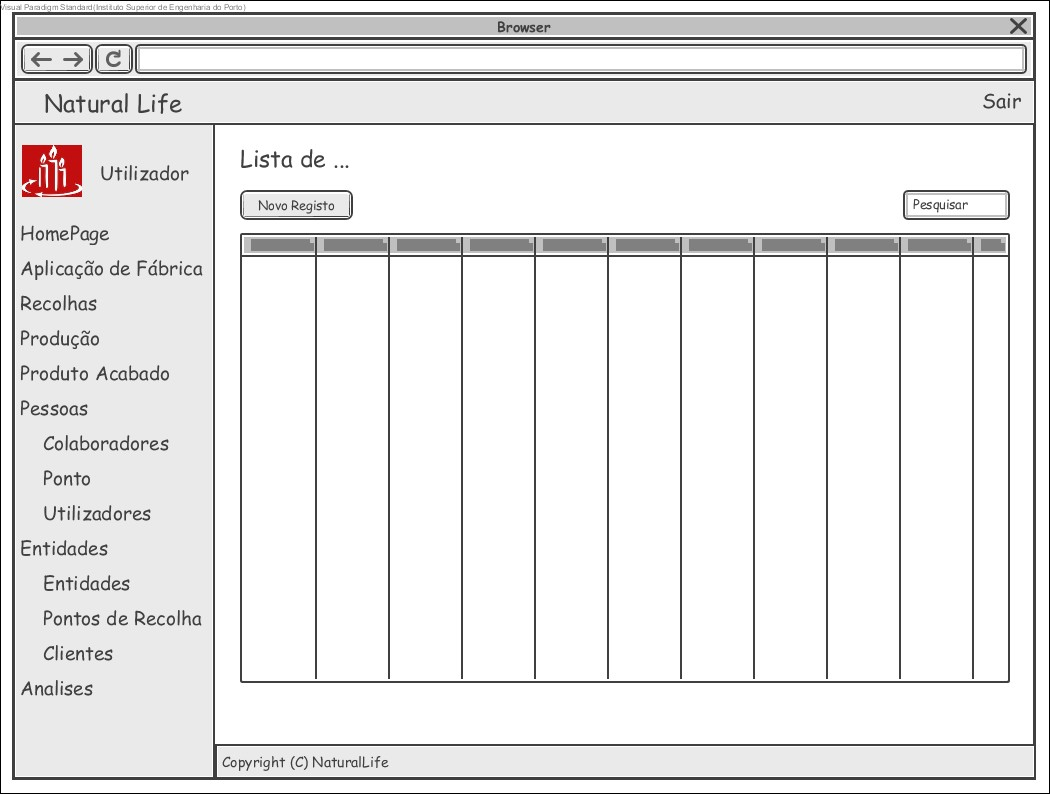
\includegraphics[width=0.60\textwidth,keepaspectratio]{figuras/Diagramas_vp/DI_Painel_1_Lista.jpg}
		\caption{Modelo da página de listagem}
		\label{fig:di_lista} 
	\end{center}
\end{figure}

\subsubsection*{Models compatíveis com o caso de uso}
Todos os models são compatíveis com este caso de uso

\subsubsection*{Fluxo do caso de utilização}
O caso de uso inicia-se com a abertura da página de listagem. É apresentado uma tabela com os dados listado e algumas opções para cada linha, tal como demonstrado na figura \ref{fig:sd_lista}.


\begin{figure}[H] 
	\begin{center}
		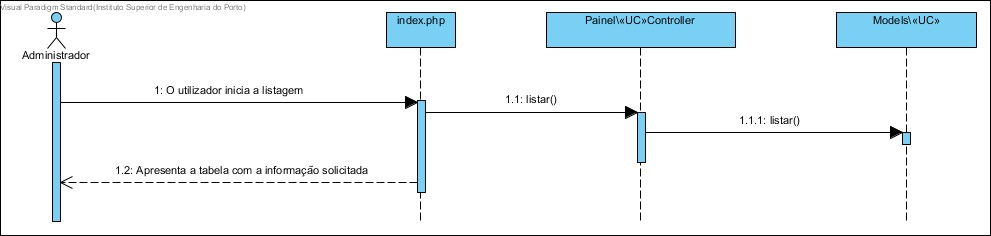
\includegraphics[width=\textwidth,keepaspectratio]{figuras/Diagramas_vp/SD_Painel_1_Listar.jpg}
		\caption{Diagrama de sequência da listagem}
		\label{fig:sd_lista} 
	\end{center}
\end{figure}